\subsection{Модели упругого рассеяния электронов в веществе}
Упругое рассеяние происходит в основном в результате взаимодействия высокоэнергетических электронов с ядрами атомов, частично экранированными их электронами. При этом изменяется направление движения электрона, а его энергия остается практически неизменной. Азимутальный угол рассеяния $\phi$ распределен равномерно в промежутке (0$^\circ$, 360$^\circ$), полярный угол рассеяния $\theta$ распределен в промежутке (0$^\circ$ до 180$^\circ$) со средним значением 5$^\circ$-10$^\circ$.

Основной характеристикой упругого рассеяния электронов на атомах вещества является дифференциальное сечение рассеяния $\frac{d \sigma}{d \Omega}$, определяемое как отношение числа электронов, рассеянных мишенью в элемент телесного угла $d \Omega = d \varphi \sin \theta d \theta$ за единицу времени, к плотности потока электронов. Полное сечение упругого рассеяния определяется как интеграл от дифференциального сечения по полному телесному углу:
\begin{equation} \label{eq:models_1}
	\sigma_\mathrm{el}=2 \pi \int_0^\pi \frac{d \sigma}{d \Omega} \sin \theta d \theta.
\end{equation}

\subsubsection{Формула Резерфорда}
Для определения дифференциального сечения упругого рассеяния электронов на атомах вещества можно воспользоваться формулой Резерфорда~\cite{Dapor_large_book}:
\begin{equation} \label{eq:models_3}
	\frac{d \sigma_\mathrm{R}}{d \Omega}=\frac{Z^2 e^4}{4 E^2(1-\cos \theta+2 \beta)^2},
\end{equation}
где $Z$ -- зарядовое число атомов вещества, $e$ -- заряд электрона, $E$ -- энергия налетающего электрона, $\beta$ -- параметр экранирования. Формула Резерфорда хорошо описывает сечения упругого рассеяния электронов на легких атомах, однако, ее точность снижается с ростом зарядового числа атомов, особенно, в области низких энергий (<1 кэВ)~\cite{Dapor_large_book}.

\subsubsection{Моттовские сечения}
Более точные значения сечений упругого рассеяния (моттовские сечения) могут быть получены за счет решения уравнения Дирака для задачи рассеяния релятивистского электрона в центральном статическом поле атома-мишени~\cite{Czyzewski_mott_cs}. В этом подходе дифференциальное сечение упругого рассеяния задается формулой
\begin{equation}
	\frac{d \sigma_\mathrm{el}}{d \Omega}=|f(\theta)|^2+|g(\theta)|^2,
\end{equation}
где $f(\theta)$ и $g(\theta)$ -- амплитуды рассеяния, соответствующие параллельному и антипараллельному направлению спина электрона относительно его направления движения соответственно и определяемые следующими выражениями:
\begin{equation}
	\begin{aligned}
		&f(\theta)=\frac{1}{2 i K} \sum_{l=0}^{\infty}\left\{(l+1)\left[\exp \left(2 i \delta_l^{-}\right)-1\right]+l\left[\exp \left(2 i \delta_l^{+}\right)-1\right]\right\} P_l(\cos \theta), \\
		&g(\theta)=\frac{1}{2 i K} \sum_{l=0}^{\infty}\left[-\exp \left(2 i \delta_l^{-}\right)+\exp \left(2 i \delta_l^{+}\right)\right] P_l^1(\cos \theta).
	\end{aligned}
\end{equation}
Здесь $k$ -- волновое число налетающего релятивистского электрона, $P_l(\cos \theta)$ и $P_l^1 (\cos \theta)$ -- полиномы Лежандра и присоединенные полиномы Лежандра соответственно, $\delta_l^{\pm}$ -- фазовые сдвиги сферических волн, рассчитываемые по формуле
\begin{equation}
	\tg \left(\delta_l^{\pm}\right)=\frac{K j_{l+1}(K r)-j_l(K r)\left[(W+1) \tg \phi_l^{\pm}+\left(1+l+k^{\pm}\right) / r\right]}{K n_{l+1}(K r)-n_l(K r)\left[(W+1) \tg \phi_l^{\pm}+\left(1+l+k^{\pm}\right) / r\right]},
\end{equation}
где $K^2 = W^2 - 1$ , $W$ -- полная энергия электрона в единицах $mc^2$, $r$ -- расстояние до рассеивающего центра в единицах $h/2 \pi mc$. 
Индексы ``+'' и ``0'' обозначают параллельное и антипараллельное направление спина, соответственно:
\begin{equation}
	\begin{aligned}
		&+: k^{+}=-l-1, \quad & j=l+1 / 2, \\
		&-: k^{-}=l, \quad & j=l-1 / 2 .
	\end{aligned}
\end{equation}
При этом $\phi_l^\pm$ -- предел функции $\phi_l^\pm (r)$ (при $r \rightarrow \infty$), которая находится путем численного интегрирования уравнения Дирака:
\begin{equation}
	\frac{d \phi_l^{\pm}(r)}{d r}=\frac{k^{\pm}}{r} \sin \left[2 \phi_l^{\pm}(r)\right]-\cos \left[2 \phi_l^{\pm}(r)\right]+W-V(r),
\end{equation}
где $V(r)$ -- рассеивающий потенциал.


\subsection{Модели квазиупругого рассеяния электронов в веществе}
\subsubsection{Модель электрон-фононного рассеяния}
За счет теплового движения атомы кристаллических тел колеблются вблизи своих положений равновесия. С такими колебаниями связывается наличие фононов в кристаллической решетке, и их число может изменяться за счет взаимодействия налетающего электрона с оптическими модами колебаний решетки~\cite{Fronlich_phonons, Llacer_phonons}. Энергия фононов не превышает значения $\kB T_\mathrm{D}$, где $\kB$ -- постоянная Больцмана и $T_\mathrm{D}$ -- температура Дебая. Для большинства твердых тел величина $\kB T_\mathrm{D}$ составляет менее 0.1 эВ, и учет потерь энергии налетающего электрона за счет генерации фононов становится целесообразен при энергиях электрона порядка 1~эВ~\cite{Ganachaud_phonons_polarons}.

Согласно существующим работам~\cite{Fronlich_phonons, Llacer_phonons}, обратная длина свободного пробега при электрон-фононном рассеянии может быть выражена формулой
\begin{equation} \label{eq:phonons}
	\lambda_{\mathrm{ph}}^{-1}=\frac{1}{a_0} \frac{\varepsilon_0-\varepsilon_{\infty}}{\varepsilon_0 \varepsilon_{\infty}} \frac{\hbar \omega}{E} \frac{n(T)+1}{2} \ln \left[\frac{1+\sqrt{1-\hbar \omega / E}}{1-\sqrt{1-\hbar \omega / E}}\right],
\end{equation}
где $E$ -- энергия налетающего электрона, $\hbar \omega$ -- его потери энергии (порядка 0.01–0.1 эВ), $\varepsilon_0$ -- статическая диэлектрическая проницаемость, $\varepsilon_\infty$ -- высокочастотная диэлектрическая проницаемость, $a_0$ -- боровский радиус и $n(T)$ -- число заполнения:
\begin{equation}
	n(T)=\frac{1}{e^{\hbar \omega / kB T}-1},
\end{equation}
где $\kB$ -- постоянная Больцмана. Было установлено, что для ПММА величина $\hbar \omega$ может быть принята равной 0.1 эВ~\cite{Fronlich_phonons, Llacer_phonons}, что вкупе с формулой~\ref{eq:phonons} предоставляет все необходимое для моделирования электрон-фононного взаимодействия.


\subsubsection{Модель электрон-поляронного рассеяния}
Электроны, медленно движущиеся в диэлектриках, приводят к появлению поляризационного поля, которое оказывает на них стабилизирующее воздействие. Такой процесс описывается как генерация квазичастицы – полярона, состоящего из электрона и поляризационного облака вокруг него. Было установлено, что энергетическая зависимость обратной длины свободного пробега электрона при таком взаимодействии может быть описана экспоненциальной функцией~\cite{Ganachaud_phonons_polarons}:
\begin{equation}
	\lambda_\mathrm{pol}^{-1}=C e^{-\gamma E}.
\end{equation}
Параметры $C$ и $\gamma$ определяются косвенным методом (например, путем анализа различных распределений для вторичных электронов~\cite{Ciappa_2010, Dapor2011}). При этом считается, что при генерации полярона налетающий электрон полностью останавливается ($\hbar \omega = E$). Было установлено, что для ПММА параметры $C$ и $\gamma$ могут быть приняты равными 0.1 нм$^\text{-1}$ и 0.15 эВ$^\text{-1}$ соответственно~\cite{Dapor_large_book}. Следует отметить, что в силу фиксированных потерь энергии как при электрон-фононном, так и при электрон-поляронном рассеянии допустимо непосредственное использование обратной длины свободного пробега (без предварительного вычисления дифференциальной обратной длины свободного пробега).


\subsection{Модели неупругого рассеяния электронов в веществе}
Квазиупругие и неупругие процессы включают в себя все процессы взаимодействия между налетающим электроном и веществом мишени, в которых электрон теряет свою энергию. При этом также происходит изменение направления движения электрона, и полярный угол рассеяния $\theta$ задается выражением~\cite{Ciappa_2010}
\begin{equation}
	\sin ^2 \theta=\frac{\hbar \omega}{E},
\end{equation}
где $E$ -- энергия электрона до акта рассеяния, $\hbar \omega$ -- потери энергии. В моделях неупругого рассеяния часто рассматривается взаимодействие налетающего электрона с веществом мишени в целом, и для описания такого взаимодействия используется обратная длина свободного пробега $\lambda_\mathrm{inel}^{-1}(E)$, связанная с сечением неупругого рассеяния формулой
\begin{equation}
	\lambda_{\text{inel}}^{-1}(E) = n \sigma(E),
\end{equation}
где $n$ -- концентрация рассеивающих центров в веществе.


\subsubsection{Модель непрерывных потерь энергии}
Исторически первые подходы к описанию потерь энергии электрона в веществе основывались на формуле Бете~\cite{Bethe}:
\begin{equation}
	-\left(\frac{d E}{d s}\right)_{\text {Bethe }}=2 \pi e^4 N_\mathrm{A} \frac{\rho}{Z} \frac{1}{E} \ln \left(\frac{1.66 E}{J}\right),
\end{equation}
где $N_\mathrm{A}$ -- число Авогадро, $\rho$ -- плотность вещества, $Z$ -- порядковый номер атомов вещества, $e$ и $E$ -- заряд и энергия движущегося в веществе электрона соответственно. Средний потенциал ионизации $J$ определяется экспериментально или вычисляется на основе порядкового номера атомов вещества~\cite{Dapor_large_book}:
\begin{equation}
	\frac{J}{Z} = 9.76 + 58.8 Z^{-1.19}.
\end{equation}
Формула Бете с высокой точностью описывает потери энергии в области высоких энергий налетающего электрона ($E \gg J$). Однако, при приближении энергии налетающего электрона к среднему потенциалу ионизации точность формулы снижается, а в области $E < J$ потери энергии, рассчитываемые по ней, становятся отрицательными. Существуют модификации формулы Бете, позволяющие использовать ее в области низких энергий, в которых потери энергии при $E \rightarrow 0$ описываются степенной функцией~\cite{Bethe_corrected}:
\begin{equation}
	-\frac{dE}{ds} \propto \frac{1}{\sqrt{E}}.
\end{equation}
В таком виде формула Бете может быть использована, например, для оценки количества обратно отраженных и вторичных электронов, что дает правдоподобные результаты~\cite{Bethe_corr_2ndary_e}. Однако, неограниченный рост потерь энергии при $E \rightarrow 0$ противоречит эмпирическим данным, согласно которым при уменьшении энергии налетающего электрона его потери энергии достигают максимума при энергии в несколько сотен электрон вольт, затем стремятся к нулю~\cite{Shimizu_Review}.


\subsubsection{Модель дискретных потерь энергии}
В современных моделях неупругого рассеяния потери энергии электрона в веществе сводятся к дискретным процессам. В них, аналогично случаю с упругим рассеянием, вводится дифференциальная обратная длина свободного пробега $\frac{d \lambda_\mathrm{inel}^{-1}}{d \hbar \omega}(E, \hbar \omega)$, позволяющая определить обратную длину свободного пробега по формуле~\cite{Dapor_large_book}
\begin{equation}
	\lambda_\mathrm{inel}^{-1}(E)=\int_0^{E / 2} \frac{d \lambda_{\text {inel }}^{-1}(E, \hbar \omega)}{d \hbar \omega} d \hbar \omega,
\end{equation}
а также потери энергии электрона на единицу длины пути $\frac{dE}{ds}$ по формуле
\begin{equation}
	\frac{dE}{ds}(E) = \int_0^{E / 2} \frac{d \lambda_\mathrm{inel}^{-1}(E, \hbar \omega)}{d \hbar \omega} \hbar \omega d \hbar \omega.
\end{equation}
Потери энергии $\hbar \omega$ при неупругом рассеянии также определяются на основе функции $\frac{d \lambda_\mathrm{inel}^{-1}}{d \hbar \omega}$  методом Монте-Карло~\cite{Ciappa_2010}.

Наиболее распространенный подход к определению дифференциальной обратной длины свободного пробега основан на использовании функции потерь энергии (Energy Loss Function, ELF)~\cite{Dapor_large_book}:
\begin{equation}
	\operatorname{ELF}(q, \omega) \equiv \operatorname{Im}\left[\frac{-1}{\varepsilon(q, \omega)}\right].
\end{equation}
Здесь $\varepsilon(q, \omega)$ -- комплексная диэлектрическая функция, $\vec{q}$ и $\hbar \omega$ -- передаваемые среде импульс и энергия соответственно. При известной функции потерь энергии дифференциальная обратная длина свободного пробега может быть найдена по формуле
\begin{equation}
	\frac{d \lambda_{\text {inel }}^{-1}}{d \hbar \omega}=\frac{1}{\pi E a_0} \int_{k_{-}}^{k_{+}} \operatorname{Im}\left[\frac{-1}{\varepsilon(q, \omega)}\right] \frac{d q}{q},
\end{equation}
где
\begin{equation}
	q_{\pm}=\frac{\sqrt{2 m}}{\hbar}(\sqrt{E} \pm \sqrt{E-\hbar \omega}),
\end{equation}
$E$ -- энергия налетающего электрона, $m$ -- масса электрона и $a_0$ -- боровский радиус.

Поскольку функция $\varepsilon(q, \omega)$ может быть найдена из первых принципов только в некоторых идеализированных случаях~\cite{Ritchie_ELF}, часто используется подход на основе оптической функции потерь энергии (Optical Energy Loss Function, OELF), получаемой в пределе $q \rightarrow 0$:
\begin{equation}
	\operatorname{OELF}(\omega) \equiv E L F(0, \omega)=\operatorname{Im}\left[\frac{-1}{\varepsilon(0, \omega)}\right].
\end{equation}
Оптическая функция потерь энергии может быть рассчитана на основе значений коэффициентов преломления ($n$) и поглощения ($k$)~\cite{Dapor_2015_oscillators} (рисунок~\ref{fig:OLF}a):
\begin{equation}
	\operatorname{Im}\left[\frac{-1}{\varepsilon(0, \omega)}\right]=\frac{2 n k}{\left(n^2+k^2\right)^2}.
\end{equation}
Коэффициенты $n$ и $k$ табулированы для многих веществ в области низких энергий (примерно до 2~кэВ)~\cite{Palik}, для более высоких энергий они могут быть определены из компонент атомных факторов рассеяния $f = f_1 + i f_2$ (для молекулярных веществ)~\cite{Henke_photoabs}:
\begin{equation}
	\begin{aligned}
		&n=1-\frac{e^2}{2 \pi m c^2} \lambda^2 N \sum_p x_p f_{1 p}, \\
		&k=\frac{e}{2 \pi m c^2} \lambda^2 N \sum_p x_p f_{2 p}.
	\end{aligned}
\end{equation}
Здесь $N$ -- концентрация молекул, содержащих $x_p$ атомов каждого вида, $\lambda$ -- длина волны фотона. Для атомарных веществ оптическая функция потерь энергии может быть найдена непосредственно по формуле
\begin{equation}
	\operatorname{Im}\left[\frac{-1}{\varepsilon(0, \omega)}\right]=\frac{n_\mathrm{c} c \sigma_\mathrm{phot}}{\omega},
\end{equation}
где $n_\mathrm{c}$ -- концентрация остовных электронов, $\sigma_\mathrm{phot}$ --  сечение фотоионизации~\cite{Biggs_cs}. При известной оптической функции потерь энергии поведение функция потерь энергии в области $q > 0$ учитывается с помощью одного из подходов, описанных ниже.


\paragraph{Аппроксимация функции потерь энергии эмпирической функцией} \mbox{} \\
\indent Наиболее простым является подход, в котором поведение функции потерь энергии в области $q > 0$ учитывается за счет использования эмпирических функций $L(x)$ и $S(x)$, что позволяет непосредственно рассчитать обратную длину свободного пробега~\cite{Ashley_LxSx}
\begin{equation}
	\begin{aligned}
		&\lambda^{-1}(E)=\frac{m e^2}{2 \pi \hbar^2 E} \int_0^{W_{\max }} \operatorname{Im}\left[\frac{-1}{\varepsilon(0, \omega)}\right] L\left(\frac{\hbar \omega}{E}\right) d \hbar \omega, \\
		&L(x)=(1-x) \ln \frac{4}{x}-\frac{7}{4} x+x^{3 / 2}-\frac{33}{32} x^2,
	\end{aligned}
\end{equation}
а также потери энергии на единицу длины пути
\begin{equation}
	\begin{aligned}
		&\lambda^{-1}(E)=\frac{m e^2}{2 \pi \hbar^2 E} \int_0^{W_{\max }} \operatorname{Im}\left[\frac{-1}{\varepsilon(0, \omega)}\right] L\left(\frac{\hbar \omega}{E}\right) d \hbar \omega, \\
		&L(x)=(1-x) \ln \frac{4}{x}-\frac{7}{4} x+x^{3 / 2}-\frac{33}{32} x^2.
	\end{aligned}
\end{equation}



\paragraph{Аппроксимация функции потерь энергии суммой осцилляторов Друде} \mbox{} \\
\indent В данном подходе оптическая функция потерь энергии приближается суммой осцилляторов Друде~\cite{Ritchie_Drude} (рисунок~\ref{fig:OLF}б):
\begin{equation}
	\operatorname{Im}\left[\frac{-1}{\varepsilon(0, \omega)}\right]=\sum_i \frac{A_i \Gamma_i \hbar \omega}{\left[E_i^2-(\hbar \omega)^2\right]^2+\left(\Gamma_i \hbar \omega\right)^2}.
\end{equation}
Параметры отдельных осцилляторов $E_i$, $\Gamma_i$ и $A_i$ определяются путем аппроксимации оптической функции потерь энергии~\cite{Dapor_2015_oscillators}, а продолжение оптической функции потерь энергии в область осуществляется за счет использования квадратичного закон дисперсии:
\begin{equation}
	E_i(q)=E_i+\frac{\hbar^2 q^2}{2 m},
\end{equation}
что в дальнейшем позволяет получить функцию потерь энергии:
\begin{equation}
	\operatorname{Im}\left[\frac{-1}{\varepsilon(q, \omega)}\right]=\sum_i \frac{A_i \Gamma_i \hbar \omega}{\left[\left(E_i+\frac{\hbar^2 q^2}{2 m}\right)^2-(\hbar \omega)^2\right]^2+\left(\Gamma_i \hbar \omega\right)^2}.
\end{equation}

\begin{figure}[t]
	\begin{minipage}{0.5\textwidth}
		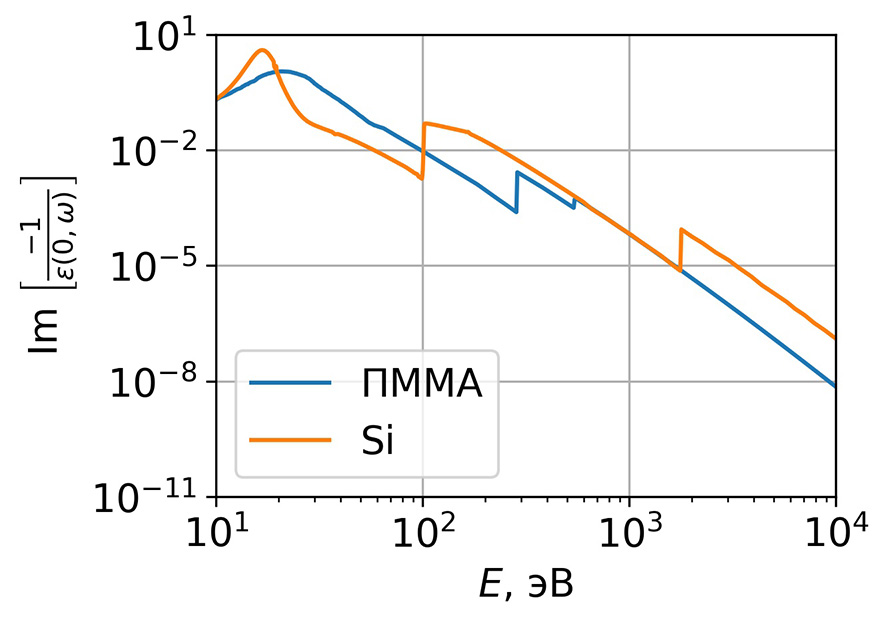
\includegraphics[width=\linewidth]{OLF/PMMA_Si_OLF_shrink_200} \\
		\vspace{-12.5em} \\ \text{\hspace{0em} a}) \\ \vspace{12.5em}
	\end{minipage}
	\begin{minipage}{0.5\textwidth}
		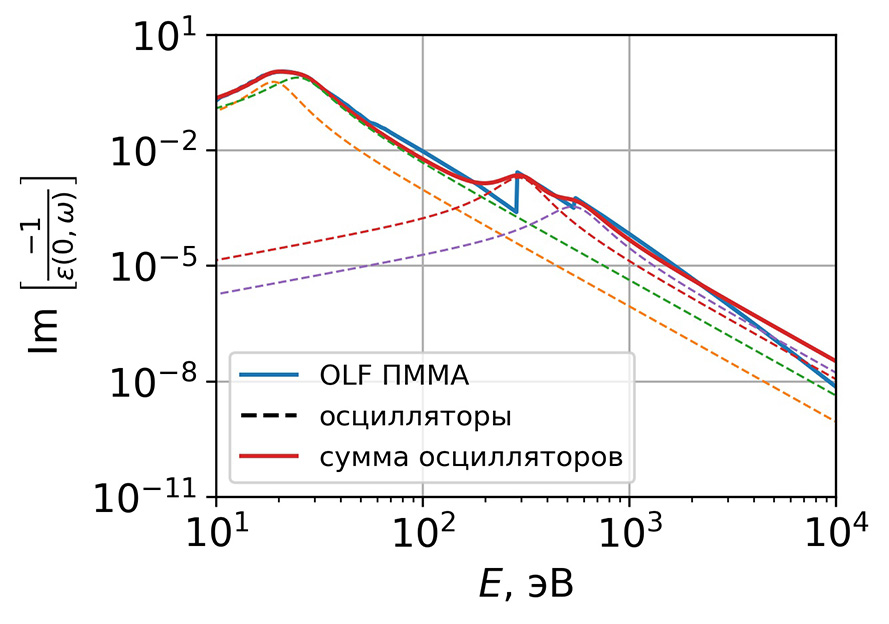
\includegraphics[width=\linewidth]{OLF/OLF_PMMA_fit_200} \\
		\vspace{-12.5em} \\ \text{\hspace{-0.1em} б}) \\ \vspace{12.5em}
	\end{minipage}
	\vspace{-3.5em}
	\caption{а) Оптическая функции потерь энергии, рассчитанная для ПММА и Si~\cite{Palik, Ritchie_ELF}; б) оптическая функция потерь энергии ПММА, приближенная суммой осцилляторов Друде~\cite{Dapor_2015_oscillators}.}
	\label{fig:OLF}
\end{figure}


\paragraph{Диэлектрическая функция Мермина} \mbox{} \\
\indent Наиболее точным подходом к определению функции потерь энергии для органических полимеров является подход на основе модели Мермина~\cite{Mermin}. В его основе лежит диэлектрическая функция Мермина для столкновительной плазмы:
\begin{equation}
	\varepsilon_\mathrm{M}(q, \omega)=1+\frac{(1+i \gamma / \omega)\left[\varepsilon_\mathrm{L}(q, \omega+i \gamma)-1\right]}{1+(i \gamma / \omega)\left[\varepsilon_\mathrm{L}(q, \omega+i \gamma)-1\right] /\left[\varepsilon_\mathrm{L}(q, 0)-1\right]},
\end{equation}
где $\gamma$ -- постоянная затухания, $\varepsilon_\mathrm{L}(q, \omega)$ -- диэлектрическая функция Линдхарда~\cite{Lindhard}:
\begin{equation}
	\varepsilon_\mathrm{L}(q, \omega)=1+\frac{\chi^2}{z^2}\left[f_1(u, z)+i f_2(u, z)\right].
\end{equation}
Здесь $u=\omega /\left(q v_\mathrm{F}\right)$, $z=q /\left( 2 q_\mathrm{F} \right)$ и $\chi^2=e^2 / \left( \pi \hbar v_\mathrm{F} \right)$, где $v_\mathrm{F}$
-- скорость Ферми валентных электронов вещества, $q_F=m v_\mathrm{F} / \hbar$. При этом функции $f_1(u, z)$ и $f_2(u, z)$ определяются формулами
\begin{equation}
	\begin{aligned}
		f_1(u, z) &=\frac{1}{2}+\frac{1}{8 z}[g(z-u)+g(z+u)], \\
		f_2(u, z) &= \begin{cases}\frac{\pi}{2} u, & z+u<1 \\
			\frac{\pi}{8 z}\left[1-(z-u)^2\right], & |z-u|<1<z+u \\
			0, & |z-u|>1\end{cases},
	\end{aligned}
\end{equation}
где
\begin{equation}
	g(x)=\left(1-x^2\right) \ln \left|\frac{1+x}{1-x}\right|.
\end{equation}

Как и в предыдущем случае, функция потерь энергии вещества описывается суммой функций потерь энергии, соответствующих отдельным осцилляторам, и ее вычисление производится в два этапа. Сначала оптическая функция потерь энергии вещества аппроксимируется суммой функций потерь энергии Мермина (осцилляторов Мермина) для $q=0$:
\begin{equation}
	\operatorname{Im}\left[\frac{-1}{\varepsilon(0, \omega)}\right]=\sum_i A_i \operatorname{Im}\left[\frac{-1}{\varepsilon_\mathrm{M}\left(\omega_i, \gamma_i, q=0, \omega\right)}\right],
\end{equation}
что позволяет получить параметры $A_i$, $\omega_i$ и $\gamma_i$ отдельных осцилляторов~\cite{DeVera_MELF_params}. Параметр $\omega_i$ определяет частоту каждого из осцилляторов, что позволяет определить значение параметра $v_\mathrm{F}$, входящего в величины $u$, $z$ и $\chi$, используемые в диэлектрической функции Линдхарда:
\begin{equation}
	\begin{aligned}
		&\omega_i=\sqrt{\frac{4 \pi n_i e^2}{m}} \Rightarrow n_i=\frac{\omega_i^2 m}{4 \pi e^2}, \\
		&v_{\mathrm{F}_i}=\frac{\hbar}{m}\left(3 \pi^2 n_i\right)^{1/3},
	\end{aligned}
\end{equation}
где $n_i$ -- концентрация электронов, соответствующая осциллятору с индексом $i$, $m$ -- масса электрона. Далее на основе параметров $A_i$, $\omega_i$ и $\gamma_i$ определяется функция потерь энергии:
\begin{equation}
	\operatorname{Im}\left[\frac{-1}{\varepsilon(q, \omega)}\right]=\sum_i A_i \operatorname{Im}\left[\frac{-1}{\varepsilon_\mathrm{M}\left(\omega_i, \gamma_i, q, \omega\right)}\right],
\end{equation}
что позволяет вычислить дифференциальную обратную длину свободного пробега.
